% MoML @ MIT 2026 (8th Molecular Machine Learning Conference).
% MoML's own style, per their "optional latex style files". NOT [review]: MoML states
% no blind-review policy and its submission form collects author names, so this build
% is NAMED -- unlike every other build of this paper.
% log_2022.sty already loads amsmath, inputenc, fontenc, url, microtype, xcolor,
% hyperref (at end of preamble, with backref) and caption. Do not double-load them.
\documentclass{article}
\usepackage{log_2022}

\usepackage{booktabs}
\usepackage{amsfonts}
\usepackage{amssymb}
\usepackage{graphicx}
\usepackage{natbib}

% Every number below comes from paper/macros.tex, regenerated from results/raw by
% analysis/tables.py. Do not write a literal result into this file.
% Generated by analysis/tables.py -- do not edit by hand.
\newcommand{\fsCostIntercept}{10.38}
\newcommand{\fsCostSlope}{11.78}
\newcommand{\fsHaarRecallKTwo}{0.450}
\newcommand{\fsHaarSpearmanKTwo}{0.676}
\newcommand{\fsHaarRecallKThree}{0.529}
\newcommand{\fsHaarSpearmanKThree}{0.781}
\newcommand{\fsHaarRecallKFour}{0.619}
\newcommand{\fsHaarSpearmanKFour}{0.859}
\newcommand{\fsHaarRecallKFive}{0.717}
\newcommand{\fsHaarSpearmanKFive}{0.916}
\newcommand{\fsHaarRecallKSix}{0.834}
\newcommand{\fsHaarSpearmanKSix}{0.962}
\newcommand{\fsHeadSubRecallKThree}{0.477}
\newcommand{\fsGaussRecallKThree}{0.304}
\newcommand{\fsTotalKThreeBOne}{1.83}
\newcommand{\fsTotalKTwoBOne}{2.31}
\newcommand{\fsIncrKThreeBOne}{2.34}
\newcommand{\fsIncrKTwoBOne}{3.51}
\newcommand{\fsTotalKThreeBSixtyFour}{1.87}
\newcommand{\fsTotalKTwoBSixtyFour}{2.39}
\newcommand{\fsIncrKThreeBSixtyFour}{2.33}
\newcommand{\fsIncrKTwoBSixtyFour}{3.51}
\newcommand{\fsGateSkipThreeBPA}{0.857}
\newcommand{\fsGateRecallThreeBPA}{0.983}
\newcommand{\fsGateSpeedupThreeBPA}{1.38}
\newcommand{\fsGateSkipEthanol}{0.777}
\newcommand{\fsGateRecallEthanol}{0.976}
\newcommand{\fsGateSpeedupEthanol}{1.32}
\newcommand{\fsGateSkipAspirin}{0.758}
\newcommand{\fsGateRecallAspirin}{0.993}
\newcommand{\fsGateSpeedupAspirin}{1.30}
\newcommand{\fsGateSkipAzobenzene}{0.845}
\newcommand{\fsGateRecallAzobenzene}{0.971}
\newcommand{\fsGateSpeedupAzobenzene}{1.37}
\newcommand{\fsNBoot}{10,000}
\newcommand{\fsHaarRecallKTwoCI}{[0.414, 0.479]}
\newcommand{\fsHaarSpearmanKTwoCI}{[0.661, 0.689]}
\newcommand{\fsHaarRecallKThreeCI}{[0.490, 0.566]}
\newcommand{\fsHaarSpearmanKThreeCI}{[0.768, 0.792]}
\newcommand{\fsHaarRecallKFourCI}{[0.580, 0.648]}
\newcommand{\fsHaarSpearmanKFourCI}{[0.850, 0.867]}
\newcommand{\fsCVRecallKFour}{0.730}
\newcommand{\fsCVRecallKFourCI}{[0.692, 0.760]}
\newcommand{\fsCVSpearmanKFour}{0.928}
\newcommand{\fsDeltaVsHeadSub}{-0.040}
\newcommand{\fsDeltaVsHeadSubCI}{[-0.074, -0.008]}
\newcommand{\fsDeltaOrtho}{0.225}
\newcommand{\fsDeltaOrthoCI}{[0.186, 0.263]}
\newcommand{\fsDeltaCV}{0.111}
\newcommand{\fsDeltaCVCI}{[0.080, 0.145]}
\newcommand{\fsBestTotalKThreeBOne}{1.11}
\newcommand{\fsBestIncrKThreeBOne}{1.63}
\newcommand{\fsBestGateSpeedupBOne}{0.93}
\newcommand{\fsBestTotalKThreeBSixteen}{1.85}
\newcommand{\fsBestIncrKThreeBSixteen}{3.18}
\newcommand{\fsBestGateSpeedupBSixteen}{1.41}
\newcommand{\fsBatchedFlatLaneOne}{25.5}
\newcommand{\fsBatchedFlatLaneEight}{30.5}
\newcommand{\fsCompileSpeedupLo}{1.04}
\newcommand{\fsCompileSpeedupHi}{1.10}
\newcommand{\fsCompileRelErr}{2.2\times10^{-7}}
\newcommand{\fsGateEnergySkipLo}{0.294}
\newcommand{\fsGateEnergySkipHi}{0.525}
\newcommand{\fsGateEnergyRecallLo}{0.636}
\newcommand{\fsGateEnergyRecallHi}{1.000}
\newcommand{\fsGateEnergySpeedLo}{1.05}
\newcommand{\fsGateEnergySpeedHi}{1.33}
\newcommand{\fsGateHeadExactSkipLo}{0.474}
\newcommand{\fsGateHeadExactSkipHi}{0.747}
\newcommand{\fsGateHeadExactRecallLo}{0.847}
\newcommand{\fsGateHeadExactRecallHi}{0.936}
\newcommand{\fsGateHeadExactSpeedLo}{1.16}
\newcommand{\fsGateHeadExactSpeedHi}{1.33}
\newcommand{\fsGateHaarSkipLo}{0.525}
\newcommand{\fsGateHaarSkipHi}{0.734}
\newcommand{\fsGateHaarRecallLo}{0.870}
\newcommand{\fsGateHaarRecallHi}{0.926}
\newcommand{\fsGateHaarSpeedLo}{1.19}
\newcommand{\fsGateHaarSpeedHi}{1.32}
\newcommand{\fsGateCVSkipLo}{0.836}
\newcommand{\fsGateCVSkipHi}{0.872}
\newcommand{\fsGateCVRecallLo}{0.964}
\newcommand{\fsGateCVRecallHi}{0.982}
\newcommand{\fsGateCVSpeedLo}{1.40}
\newcommand{\fsGateCVSpeedHi}{1.43}
\newcommand{\fsGateEnergySkipThreeBPA}{0.294}
\newcommand{\fsGateEnergyRecallThreeBPA}{0.894}
\newcommand{\fsGateEnergySpeedThreeBPA}{1.05}
\newcommand{\fsGateEnergyRecallThreeBPACI}{[0.800, 0.977]}
\newcommand{\fsGateEnergySkipThreeBPACI}{[0.269, 0.319]}
\newcommand{\fsGateEnergySkipEthanol}{0.322}
\newcommand{\fsGateEnergyRecallEthanol}{1.000}
\newcommand{\fsGateEnergySpeedEthanol}{1.07}
\newcommand{\fsGateEnergyRecallEthanolCI}{[1.000, 1.000]}
\newcommand{\fsGateEnergySkipEthanolCI}{[0.285, 0.358]}
\newcommand{\fsGateEnergySkipAspirin}{0.403}
\newcommand{\fsGateEnergyRecallAspirin}{0.867}
\newcommand{\fsGateEnergySpeedAspirin}{1.16}
\newcommand{\fsGateEnergyRecallAspirinCI}{[0.733, 0.971]}
\newcommand{\fsGateEnergySkipAspirinCI}{[0.365, 0.443]}
\newcommand{\fsGateEnergySkipAzobenzene}{0.525}
\newcommand{\fsGateEnergyRecallAzobenzene}{0.636}
\newcommand{\fsGateEnergySpeedAzobenzene}{1.33}
\newcommand{\fsGateEnergyRecallAzobenzeneCI}{[0.429, 0.833]}
\newcommand{\fsGateEnergySkipAzobenzeneCI}{[0.485, 0.565]}
\newcommand{\fsGateHeadExactSkipThreeBPA}{0.747}
\newcommand{\fsGateHeadExactRecallThreeBPA}{0.926}
\newcommand{\fsGateHeadExactSpeedThreeBPA}{1.33}
\newcommand{\fsGateHeadExactRecallThreeBPACI}{[0.896, 0.953]}
\newcommand{\fsGateHeadExactSkipThreeBPACI}{[0.730, 0.764]}
\newcommand{\fsGateHeadExactSkipEthanol}{0.474}
\newcommand{\fsGateHeadExactRecallEthanol}{0.924}
\newcommand{\fsGateHeadExactSpeedEthanol}{1.16}
\newcommand{\fsGateHeadExactRecallEthanolCI}{[0.875, 0.967]}
\newcommand{\fsGateHeadExactSkipEthanolCI}{[0.449, 0.499]}
\newcommand{\fsGateHeadExactSkipAspirin}{0.643}
\newcommand{\fsGateHeadExactRecallAspirin}{0.847}
\newcommand{\fsGateHeadExactSpeedAspirin}{1.26}
\newcommand{\fsGateHeadExactRecallAspirinCI}{[0.775, 0.910]}
\newcommand{\fsGateHeadExactSkipAspirinCI}{[0.618, 0.667]}
\newcommand{\fsGateHeadExactSkipAzobenzene}{0.600}
\newcommand{\fsGateHeadExactRecallAzobenzene}{0.936}
\newcommand{\fsGateHeadExactSpeedAzobenzene}{1.23}
\newcommand{\fsGateHeadExactRecallAzobenzeneCI}{[0.896, 0.971]}
\newcommand{\fsGateHeadExactSkipAzobenzeneCI}{[0.573, 0.627]}
\newcommand{\fsGateHaarSkipThreeBPA}{0.734}
\newcommand{\fsGateHaarRecallThreeBPA}{0.926}
\newcommand{\fsGateHaarSpeedThreeBPA}{1.32}
\newcommand{\fsGateHaarRecallThreeBPACI}{[0.898, 0.951]}
\newcommand{\fsGateHaarSkipThreeBPACI}{[0.717, 0.752]}
\newcommand{\fsGateHaarSkipEthanol}{0.525}
\newcommand{\fsGateHaarRecallEthanol}{0.912}
\newcommand{\fsGateHaarSpeedEthanol}{1.19}
\newcommand{\fsGateHaarRecallEthanolCI}{[0.856, 0.963]}
\newcommand{\fsGateHaarSkipEthanolCI}{[0.500, 0.550]}
\newcommand{\fsGateHaarSkipAspirin}{0.548}
\newcommand{\fsGateHaarRecallAspirin}{0.870}
\newcommand{\fsGateHaarSpeedAspirin}{1.20}
\newcommand{\fsGateHaarRecallAspirinCI}{[0.824, 0.912]}
\newcommand{\fsGateHaarSkipAspirinCI}{[0.524, 0.572]}
\newcommand{\fsGateHaarSkipAzobenzene}{0.553}
\newcommand{\fsGateHaarRecallAzobenzene}{0.914}
\newcommand{\fsGateHaarSpeedAzobenzene}{1.21}
\newcommand{\fsGateHaarRecallAzobenzeneCI}{[0.869, 0.952]}
\newcommand{\fsGateHaarSkipAzobenzeneCI}{[0.526, 0.580]}
\newcommand{\fsGateCVSkipThreeBPA}{0.844}
\newcommand{\fsGateCVRecallThreeBPA}{0.972}
\newcommand{\fsGateCVSpeedThreeBPA}{1.41}
\newcommand{\fsGateCVRecallThreeBPACI}{[0.949, 0.991]}
\newcommand{\fsGateCVSkipThreeBPACI}{[0.828, 0.860]}
\newcommand{\fsGateCVSkipEthanol}{0.836}
\newcommand{\fsGateCVRecallEthanol}{0.982}
\newcommand{\fsGateCVSpeedEthanol}{1.40}
\newcommand{\fsGateCVRecallEthanolCI}{[0.940, 1.000]}
\newcommand{\fsGateCVSkipEthanolCI}{[0.812, 0.859]}
\newcommand{\fsGateCVSkipAspirin}{0.851}
\newcommand{\fsGateCVRecallAspirin}{0.973}
\newcommand{\fsGateCVSpeedAspirin}{1.41}
\newcommand{\fsGateCVRecallAspirinCI}{[0.946, 0.994]}
\newcommand{\fsGateCVSkipAspirinCI}{[0.828, 0.873]}
\newcommand{\fsGateCVSkipAzobenzene}{0.872}
\newcommand{\fsGateCVRecallAzobenzene}{0.964}
\newcommand{\fsGateCVSpeedAzobenzene}{1.43}
\newcommand{\fsGateCVRecallAzobenzeneCI}{[0.926, 0.992]}
\newcommand{\fsGateCVSkipAzobenzeneCI}{[0.849, 0.894]}
\newcommand{\fsNDesignThreeBPA}{427}
\newcommand{\fsNCalThreeBPA}{428}
\newcommand{\fsNTestThreeBPA}{1284}
\newcommand{\fsNDesignEthanol}{200}
\newcommand{\fsNCalEthanol}{200}
\newcommand{\fsNTestEthanol}{600}
\newcommand{\fsNDesignAspirin}{200}
\newcommand{\fsNCalAspirin}{200}
\newcommand{\fsNTestAspirin}{600}
\newcommand{\fsNDesignAzobenzene}{200}
\newcommand{\fsNCalAzobenzene}{200}
\newcommand{\fsNTestAzobenzene}{600}
\newcommand{\fsTestPrevalenceLo}{0.028}
\newcommand{\fsTestPrevalenceHi}{0.050}
\newcommand{\fsFallbackLanesSketch}{3}
\newcommand{\fsFallbackLanesEnergy}{7}
\newcommand{\fsGateCVSkipLoPct}{84}
\newcommand{\fsGateCVSkipHiPct}{87}
\newcommand{\fsGateCVRecallLoPct}{96}
\newcommand{\fsGateCVRecallHiPct}{98}
\newcommand{\fsGateCVDominates}{11}
\newcommand{\fsGateCVComparisons}{12}
\newcommand{\fsMaxNSystems}{4}
\newcommand{\fsMaxRecallKTwoLo}{0.272}
\newcommand{\fsMaxRecallKTwoHi}{0.410}
\newcommand{\fsMaxSpearmanKTwoLo}{0.385}
\newcommand{\fsMaxSpearmanKTwoHi}{0.569}
\newcommand{\fsMaxRecallKThreeLo}{0.362}
\newcommand{\fsMaxRecallKThreeHi}{0.489}
\newcommand{\fsMaxSpearmanKThreeLo}{0.531}
\newcommand{\fsMaxSpearmanKThreeHi}{0.686}
\newcommand{\fsMaxRecallKFourLo}{0.484}
\newcommand{\fsMaxRecallKFourHi}{0.570}
\newcommand{\fsMaxSpearmanKFourLo}{0.648}
\newcommand{\fsMaxSpearmanKFourHi}{0.781}
\newcommand{\fsMaxRecallKFiveLo}{0.578}
\newcommand{\fsMaxRecallKFiveHi}{0.681}
\newcommand{\fsMaxSpearmanKFiveLo}{0.768}
\newcommand{\fsMaxSpearmanKFiveHi}{0.866}
\newcommand{\fsMaxRecallKSixLo}{0.724}
\newcommand{\fsMaxRecallKSixHi}{0.801}
\newcommand{\fsMaxSpearmanKSixLo}{0.883}
\newcommand{\fsMaxSpearmanKSixHi}{0.934}
\newcommand{\fsMaxBiasKOneLo}{1.42}
\newcommand{\fsMaxBiasKOneHi}{1.53}
\newcommand{\fsMaxBiasKFourLo}{1.07}
\newcommand{\fsMaxBiasKFourHi}{1.08}
\newcommand{\fsMaxRecallKSixLoPct}{72}
\newcommand{\fsMaxRecallKSixHiPct}{80}
\newcommand{\fsMaxRecallKFourLoPct}{48}
\newcommand{\fsMaxRecallKFourHiPct}{57}
\newcommand{\fsMaxBiasExact}{1.000}
\newcommand{\fsSerialTotalKThreeBOne}{1.83}
\newcommand{\fsSerialTotalKThreeBFour}{1.82}
\newcommand{\fsSerialTotalKThreeBSixteen}{1.85}
\newcommand{\fsSerialTotalKThreeBSixtyFour}{1.86}
\newcommand{\fsBatchedWinBOne}{3.63}
\newcommand{\fsBatchedWinBFour}{3.71}
\newcommand{\fsBatchedWinBSixteen}{1.58}
\newcommand{\fsBatchedWinBSixtyFour}{0.82}
\newcommand{\fsBatchedLosesBatch}{64}
\newcommand{\fsBatchedRatioLost}{1.22}
\newcommand{\fsKernElemExact}{42.2}
\newcommand{\fsKernElemSketchLo}{41.5}
\newcommand{\fsKernElemSketchHi}{41.9}
\newcommand{\fsKernTPExact}{21.3}
\newcommand{\fsKernTPSketchLo}{20.0}
\newcommand{\fsKernTPSketchHi}{20.9}
\newcommand{\fsKernDistinct}{134}
\newcommand{\fsKernLaunchRatio}{2.12}
\newcommand{\fsKernLaneRatio}{2.33}
\newcommand{\fsDeltaVsHeadSubAspirin}{-0.070}
\newcommand{\fsDeltaVsHeadSubAspirinCI}{[-0.126, -0.016]}
\newcommand{\fsDeltaVsHeadSubNoMeanAspirin}{-0.068}
\newcommand{\fsDeltaVsHeadSubNoMeanAspirinCI}{[-0.102, -0.016]}
\newcommand{\fsDeltaVsHeadSubThreeBPA}{-0.040}
\newcommand{\fsDeltaVsHeadSubThreeBPACI}{[-0.074, -0.008]}
\newcommand{\fsDeltaVsHeadSubNoMeanThreeBPA}{-0.059}
\newcommand{\fsDeltaVsHeadSubNoMeanThreeBPACI}{[-0.093, -0.023]}
\newcommand{\fsSeedSdLo}{0.02}
\newcommand{\fsSeedSdHi}{0.09}
\newcommand{\fsSrankLo}{2.91}
\newcommand{\fsSrankHi}{3.08}
\newcommand{\fsTopEigLo}{0.325}
\newcommand{\fsTopEigHi}{0.344}
\newcommand{\fsTopEigIsotropic}{0.143}
\newcommand{\fsTopEigRatioLo}{2.3}
\newcommand{\fsTopEigRatioHi}{2.4}


\title[Force sketching in MD]{Force sketching in MD: can a few random probes replace
multi-head committee force uncertainty?}

\author[I. Poon]{Ian Poon \\
  \institute{Department of Cellular and Molecular Biology \\ Harvard University} \\
  \email{ian\_poon@fas.harvard.edu}}

\begin{document}
\maketitle

\begin{abstract}
Committee disagreement is the standard uncertainty signal for machine-learned interatomic
potentials, and a multi-head committee makes it nearly free for \emph{energies}: $M$ heads share one
trunk, so a single forward pass returns all $M$. Forces are not free. Forces are gradients, so each
head's forces need their own backward pass, and force disagreement --- the quantity acquisition
actually consumes --- costs about $M$ times more. We ask whether $K\ll M$ cheap random probes can
estimate it instead, on a pretrained eight-head MACE committee across 3BPA and three rMD17
molecules. The answer is \emph{no} for replacement and \emph{yes} for screening. Even given six of
the seven probes the exact computation would use, the best estimator recovers only
\fsMaxRecallKSixLoPct--\fsMaxRecallKSixHiPct\% of the genuinely most uncertain structures, and we
diagnose why: the maximum over $3N$ noisy component estimates is biased upward, which no marginal
finite-$K$ correction removes. But a conformally calibrated gate built from the same cheap score
skips \fsGateCVSkipLoPct--\fsGateCVSkipHiPct\% of the expensive computations while still catching
\fsGateCVRecallLoPct--\fsGateCVRecallHiPct\%, beating a free energy-disagreement gate and head
subsampling at matched budget in \fsGateCVDominates{} of \fsGateCVComparisons{} comparisons. We
report the wall-clock caveat plainly: the saving is $\fsBestTotalKThreeBSixteen\times$ in batch but
only $\fsBestTotalKThreeBOne\times$ at batch size one, which is the single-trajectory MD regime.
\end{abstract}

\section{Why force uncertainty is the expensive half}
Uncertainty quantification is what makes a learned potential usable beyond its training
distribution: it flags extrapolation during molecular dynamics and decides when a structure must go
back to the quantum-chemistry calculation the model was trained to imitate. Committee disagreement
remains the most widely used estimator of that error --- where training data pinned the model down
its members agree, and where it did not they diverge, so their spread stands in for an error we
cannot see~\citep{behler2015,podryabinkin2017,carrete2023}. Multi-head
committees~\citep{beck2025mhc}, and shallow ensembles more broadly~\citep{kellner2024}, make this
cheap by attaching $M$ readout heads to one shared message-passing trunk, so all $M$ energies come
from a single forward pass instead of $M$ separately trained models.

That amortization does not extend to forces. As the multi-head committee work states directly, ``a
single backward pass can not yield the forces for all the heads \ldots\ the standard deviation
requires multiple reverse passes through the computational graph.'' Forces are what MD and most
acquisition rules consume, so the expensive half of committee uncertainty is exactly the half the
shared trunk fails to amortize. Downstream, though, one rarely needs every member force: acquisition
needs a \emph{ranking} and a safety gate needs a \emph{threshold decision}. That motivates estimating
the disagreement statistic directly rather than reconstructing the member forces that define it.

\section{Sketching the centered head subspace}
\label{sec:method}
For a structure of $N$ atoms with coordinates $x\in\mathbb{R}^{D}$, $D=3N$, the committee returns
head energies $E(x)\in\mathbb{R}^{M}$ from one forward pass, and head forces
$f_m=-\nabla_x E_m$ collected as columns of $F\in\mathbb{R}^{D\times M}$. With
$P=I_M-\tfrac1M\mathbf 1\mathbf 1^{\mathsf T}$ the centering projector, the per-coordinate
disagreement and its per-structure sum are
\begin{equation}
v_d=\frac{1}{M-1}\sum_{m=1}^{M}\bigl(F_{dm}-\bar F_d\bigr)^2 ,
\qquad
S=\sum_{d=1}^{D} v_d=\frac{\lVert FP\rVert_F^2}{M-1} .
\end{equation}
Reverse mode returns the gradient of \emph{one scalar} per backward pass; we call one such pass a
\emph{lane}. Since $S$ depends on $F$ only through $FP$, whose columns sum to zero, it lives in an
$(M{-}1)$-dimensional centered subspace with orthonormal basis $Q$: differentiating $q_j^{\mathsf T}E$
costs one lane and returns $g_j=Fq_j$, with $v_d=\frac{1}{M-1}\sum_j g_{j,d}^{\,2}$. Exact force
uncertainty therefore costs $M$ lanes --- $M{-}1$ centered directions plus the mean force MD needs
anyway. \emph{Our question is whether downstream decisions need all $M{-}1$ of them.}

\paragraph{Probes.} Instead of all $M{-}1$ directions, probe the subspace with $K\ll M{-}1$ random
ones and rescale. Drawing $z_k\sim\mathcal N(0,I_M)$ and centering, $w_k=Pz_k$, one lane returns
$g_k=Fw_k$ and $\widehat v_d=\frac{1}{K(M-1)}\sum_k g_{k,d}^{\,2}$ is unbiased. Random probes can
overlap and waste budget, so we instead draw a Haar-uniform orthonormal $K$-frame inside the centered
subspace. Writing $r=M{-}1$, the two have relative standard deviations $\sqrt{2/K}$ and
$\sqrt{2(r-K)/(K(r+2))}$: orthogonalization multiplies estimator variance by exactly $(r-K)/(r+2)$,
a factor of $4/9$ at $K{=}3$, $M{=}8$. It costs nothing extra and is the largest single lever we
find. These estimators are the molecular-UQ instance of randomized trace and norm
estimation~\citep{hutchinson,avron2011,hutchpp}; the orthogonal variant is the head-space analogue of
orthogonal random features~\citep{yu2016orf}.

\paragraph{Control variate.} Disagreement is not spread evenly over the subspace, so probing it
obliviously wastes budget. Splitting $P=Q_{r_0}Q_{r_0}^{\mathsf T}+R$, we evaluate the $r_0$ leading
directions of a design-split average exactly and sketch only the residual with $K'=K-r_0$ Haar
probes; the estimator stays unbiased.

\paragraph{Screening instead of replacement.} If a sketch cannot \emph{replace} the exact score, it
can still certify when that score is small. Split conformal~\citep{vovk2005,crc} turns any score into
a calibrated bound from held-out data alone: form the ratios
$\eta_i=S(x_i)/(\widehat S(x_i)+\epsilon)$ on a calibration split and let $c_\alpha$ be their
$\lceil (n+1)(1-\alpha)\rceil$-th order statistic. Then $U(x)=c_\alpha\widehat S(x)$ sits above
$S(x)$ at least $1-\alpha$ of the time, so $U(x)<\tau$ \emph{certifies} that the exact score is below
the high-uncertainty threshold: skip when it is, fall back otherwise.

\section{Experiments}
\label{sec:setup}
We use the pretrained eight-head MACE~\citep{mace} committees released
with~\citet{beck2025mhc} on 3BPA~\citep{botnet3bpa} at 1200\,K and the joint rMD17~\citep{rmd17}
committee on ethanol, aspirin and azobenzene. Each system is split once into disjoint design
($20\%$, fitting the control-variate basis and the threshold $\tau$), calibration ($20\%$, fitting
$c_\alpha$ alone) and test ($60\%$) parts. Following~\citet{beck2025mhc}, structures are ranked by
the maximum disagreement over force components; we take that as primary and report the global sum as
an easier secondary. Estimator evaluation is in float64; timing is float32 on one RTX 5070 Laptop
GPU. Ten seeds are frozen before testing and none discarded; intervals are paired
bootstraps~\citep{efron} over structures with \fsNBoot{} resamples.

\section{Results}
\subsection{Replacement fails, and we can say why}
Figure~\ref{fig:recall} gives the negative result. Under the primary max-component rule the best
sketch reaches only $\fsMaxRecallKFourLo$--$\fsMaxRecallKFourHi$ top-5\% recall at $K{=}4$ and
$\fsMaxRecallKSixLo$--$\fsMaxRecallKSixHi$ even at $K{=}6$ of $7$ --- the $0.90$ line is not attained
at any budget short of the exact basis.

The mechanism is specific to extreme-value acquisition. Making each $\widehat\sigma_d$ unbiased
\emph{marginally} does not make $\max_d\widehat\sigma_d$ unbiased: a maximum over $3N$ noisy
estimates is biased upward, and the bias grows with the estimator's noise. Measured directly, the
score is inflated by $\fsMaxBiasKOneLo$--$\fsMaxBiasKOneHi$ at $K{=}1$, falling to
$\fsMaxBiasKFourLo$--$\fsMaxBiasKFourHi$ at $K{=}4$ and to \fsMaxBiasExact{} at the full basis where
the estimator is exact --- a useful check on the pipeline. This obstructs replacement but not
screening: the bias is monotone in the estimator's noise, so a scale-calibrated gate absorbs it
into $c_\alpha$.

\begin{figure}[t]
\centering
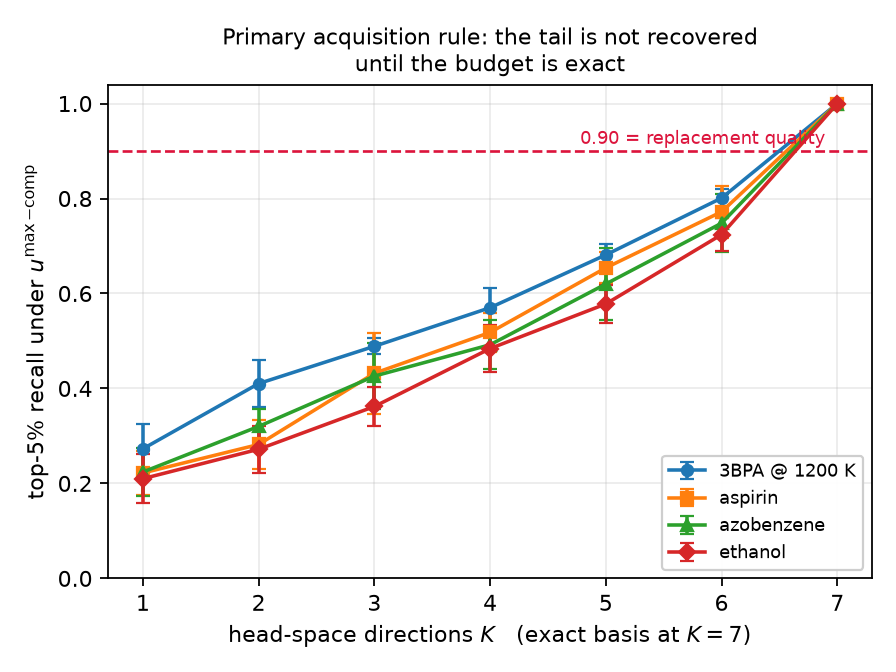
\includegraphics[width=0.52\textwidth]{figures/fig_maxcomp_recall.png}
\caption{Top-5\% recall against probe budget $K$ under the primary max-component rule, on all four
systems. Recall climbs steadily but never reaches the $0.90$ replacement line short of the exact
basis at $K{=}7$. Error bars are the standard deviation over ten frozen seeds.}
\label{fig:recall}
\end{figure}

\subsection{Screening works, and beats the cheaper gates}
A calibrated gate is a generic wrapper --- any score correlated with exact force disagreement can be
calibrated the same way --- so the claim only stands if this gate beats the cheaper ones a reader
will reach for. We build three at matched lane budget with identical splits, calibration and
threshold: a \emph{free} energy-disagreement gate (the $M$ head energies come from the forward pass
already run, costing zero uncertainty lanes); head subsampling using the \emph{exact} mean force the
sketch already pays a lane for; and a plain Haar sketch.

\begin{center}\small
\begin{tabular}{lrrrr}
\toprule
gate & lanes & exact skipped & high-UQ recall & speedup \\
\midrule
energy disagreement (free) & $1$ & \fsGateEnergySkipLo--\fsGateEnergySkipHi & \fsGateEnergyRecallLo--\fsGateEnergyRecallHi & $\fsGateEnergySpeedLo$--$\fsGateEnergySpeedHi\times$ \\
head subsampling, exact mean & $5$ & \fsGateHeadExactSkipLo--\fsGateHeadExactSkipHi & \fsGateHeadExactRecallLo--\fsGateHeadExactRecallHi & $\fsGateHeadExactSpeedLo$--$\fsGateHeadExactSpeedHi\times$ \\
Haar sketch & $5$ & \fsGateHaarSkipLo--\fsGateHaarSkipHi & \fsGateHaarRecallLo--\fsGateHaarRecallHi & $\fsGateHaarSpeedLo$--$\fsGateHaarSpeedHi\times$ \\
\textbf{control variate} & $5$ & \textbf{\fsGateCVSkipLo--\fsGateCVSkipHi} & \textbf{\fsGateCVRecallLo--\fsGateCVRecallHi} & $\mathbf{\fsGateCVSpeedLo}$--$\mathbf{\fsGateCVSpeedHi}\mathbf{\times}$ \\
\bottomrule
\end{tabular}
\end{center}
\vspace{0.3em}
{\small Ranges across the four systems, $r_0{=}2$, $K{=}4$, $\alpha{=}0.05$, on the held-out test
split. Every gate pays one mean-force lane; on fallback each completes the exact basis with $r{-}K$
further passes rather than a fresh $M$, charged identically for all of them.}
\vspace{0.3em}

The control variate \emph{Pareto-dominates} --- strictly more skipped \emph{and} strictly higher
recall --- in \fsGateCVDominates{} of the \fsGateCVComparisons{} gate-by-system comparisons,
including every one against the two sketch baselines. The exception is worth stating: on ethanol the
free energy gate attains perfect recall (\fsGateEnergyRecallEthanol{}) while skipping only
\fsGateEnergySkipEthanol. Elsewhere that free gate is the informative failure, collapsing to
\fsGateEnergyRecallAzobenzene{} recall on azobenzene --- energy disagreement is a genuinely different
signal from force disagreement, not a cheap proxy for it.

\subsection{The wall-clock caveat, stated plainly}
\label{sec:regime}
Against a \emph{batched} exact baseline the total force-plus-UQ speedup at $K{=}3$ is
$\fsBestTotalKThreeBSixteen\times$ at $B{=}16$, but collapses to $\fsBestTotalKThreeBOne\times$ at
$B{=}1$, where batched reverse mode makes extra cotangent lanes nearly free and the gate is a net
slowdown ($\fsBestGateSpeedupBOne\times$). A single MD trajectory advances one structure at a time,
so $B{=}1$ is the trajectory regime: this method pays off for batched active-learning sweeps over
candidate structures, not for stepping one trajectory. Making that baseline available at all
required disabling the TensorExpr fuser, without which batched reverse mode fails on this stack;
had we not, we would have compared against a Python loop and overstated every speedup here.

\section{Conclusion}
Exact multi-head force uncertainty cannot be replaced by a handful of randomized probes at the
fidelity acquisition requires, and the obstruction is an extreme-value bias no marginal correction
removes. It can be \emph{screened}: a conformally calibrated gate over a control-variate sketch
avoids $\fsGateCVSkipLo$--$\fsGateCVSkipHi$ of exact computations while retaining
$\fsGateCVRecallLo$--$\fsGateCVRecallHi$ of high-uncertainty structures on every system. That is a
property of the estimator; whether it saves time is a separate question whose answer is
regime-dependent. We preserve a proxy, not a demonstrated outcome: no active-learning loop is run and
no reference-force error measured, so we claim no gain in downstream model quality. Committee
disagreement is only a proxy for error; calibration is marginal and under exchangeability; $M{=}8$
bounds the maximum saving; and rMD17 spans only 9--24 atoms.

\bibliographystyle{plainnat}
\bibliography{references}

\end{document}
